\documentclass{book}
\usepackage{qtree}
\usepackage{bussproofs}
\usepackage{latexsym}
\usepackage[portugues]{algorithm2e}
\usepackage{amsmath, amsthm, amssymb}
\usepackage{url}
\usepackage{graphicx}

\usepackage[spanish]{babel}
\usepackage[utf8]{inputenc}
\newtheorem{defi}{\bf Definici\'on}
%% \newtheorem{prop}{{\bf Proposici\'on}}[chapter]
%% \newtheorem{ob}{{\bf Observaci\'on}}[chapter]
%% \newtheorem{con}{{\bf Convenci\'on}}[chapter]
%% \newtheorem{teo}{{\bf Teorema}}[chapter]
%% \newtheorem{lema}{{\bf Lema}}[chapter]
\newtheorem{ejem}{\bf Ejemplo}
%% \newtheorem{dem}{{\bf Demostración}}
%% \newcommand{\inl}{\mathop{\sf inl}}
%% \newcommand{\inr}{\mathop{\sf inr}}
%% \newcommand{\abort}{\mathop{\sf abort}}
%% \newcommand{\void}{\mathop{\sf void}}

\title {Visualizaci\'{o}n del mercado de acciones en 3D}
\author{Juan Esteban Pemberthy\\\\ Juan Sebastian Munoz}
\date{\today}
\setcounter{tocdepth}{2}

\hyphenation{subs-ti-tu-cion des-cri-ta}

\begin{document} 

\frontmatter

\maketitle
\tableofcontents
\chapter{Glosario}
\begin{enumerate}
	
\item \textbf{TDD (Test-driven development):} Desarrollo guiado por pruebas, es una práctica de programación que involucra otras dos prácticas: Escribir las pruebas primero (\textbf{Test First Development}) y Refactorización (\textbf{Refactoring}). Para escribir las pruebas generalmente se utilizan las pruebas unitarias (\textbf{unit test} en inglés). Primeramente se escribe una prueba y se verifica que las pruebas fallen, luego se implementa el código que haga que la prueba pase satisfactoriamente y seguidamente se refactoriza el código escrito. El propósito del desarrollo guiado por pruebas es lograr un código limpio que funcione (Del inglés: \textbf{Clean code that works}). La idea es que los requerimientos sean traducidos a pruebas, de este modo, cuando las pruebas pasen se garantizará que los requerimientos se hayan implementado correctamente.
\item \textbf{Pair Programming:} Programación en pareja,  requiere que dos Ingenieros en Software participen en un esfuerzo combinado de desarrollo en un sitio de trabajo. Cada miembro realiza una acción que el otro no está haciendo actualmente: Mientras que uno codifica las pruebas de unidades el otro piensa en la clase que satisfará la prueba, por ejemplo.
La persona que está haciendo la codificación se le da el nombre de controlador mientras que a la persona que está dirigiendo se le llama el navegador. Se sugiere a menudo para que a los dos socios cambien de papeles por lo menos cada media hora o después de que se haga una prueba de unidad.
\item \textbf{Mock Object:} Objeto simulado, los objetos simulados imitan el comportamiento de los objetos reales en forma controlada. Un programador generalmente escribirá un objeto simulado para probar el comportamiento de otro objeto en una forma muy similar a la que aplica un diseñador de carros al usar un muñeco para probar el comportamiento de un carro durante un accidente.
\item \textbf{RSpec:} Ruby Spec, es un framework para realizar tests en el lenguaje de programación Ruby, contiene su propio \textbf{framework} para simular objetos.
\item \textbf{ORM:} mapeo objeto-relacional, es una técnica de programación para convertir datos entre el sistema de tipos utilizado en un lenguaje de programación orientado a objetos y el utilizado en una base de datos relacional. En la práctica esto crea una base de datos orientada a objetos virtual, sobre la base de datos relacional. Esto posibilita el uso de las características propias de la orientación a objetos (básicamente herencia y polimorfismo).
\item \textbf{MVC:} Modelo Vista Controlador, es un patrón de arquitectura de software que separa los datos de una aplicación, la interfaz de usuario, y la lógica de control en tres componentes distintos. El patrón MVC se ve frecuentemente en aplicaciones web, donde la vista es la página HTML y el código que provee de datos dinámicos a la página. El modelo es el Sistema de Gestión de Base de Datos y la Lógica de negocio, y el controlador es el responsable de recibir los eventos de entrada desde la vista.
\item \textbf{Daemon:} Un demonio, (siglas en inglés, \textbf{Disk And Execution Monitor}), es un tipo especial de proceso informático que se ejecuta en segundo plano en vez de ser controlado directamente por el usuario. Este tipo de programas se ejecutan de forma continua (infinita), vale decir, que aunque se intente cerrar o matar el proceso, este continuará en ejecución o se reiniciará automáticamente. Todo esto sin intervención de terceros y sin dependencia de consola alguna.
\item \textbf{Unity3D:} Motor de Juegos para crear aplicaciones 3D.
\item \textbf{Shader:} Conjunto de instrucciones gráficas destinadas para el acelerador gráfico, estas instrucciones dan el aspecto final de un objeto. Los Shaders determinan materiales, efectos, color, luz, sombra y etc.
\item \textbf{Vertex Shaders:} Actúa sobre las coordenadas, color, textura, etc. de un vértice.
\item \textbf{Geometry Shaders:} Es capaz de generar nuevas primitivas dinamicamente.
\item \textbf{Pixel Shaders:} Actúa sobre el color de cada pixel (texel para ser más preciso).
\item \textbf{Mesh:} Término que se refiere a una figura en 3D, en general que esté formada por polígonos.
\item \textbf{Triangulación de Delaunay:} Es una red de triángulos que cumple la condición de Delaunay. Esta condición dice que la circunferencia circunscrita de cada triángulo de la red no debe contener ningún vertice de otro triángulo. Se usan triangulaciones de Delaunay en geometría por ordenar, especialmente en gráficos 3D por computadora.
\item \textbf{Transform:} Objeto en Unity3D que describe propiedades de un \textbf{Mesh} como Escalamiento, Rotación, Posición, etc.
\item \textbf{Proyección Ortográfica:} Esta proyección utliza rayos paralelos para crear una imágen de la escena. El área de vision está determinada por las longitudes de los vectores \textbf{right} y \textbf{up}, que, por cierto, han de ser especificados, ya que con este tipo de proyección no se utilizan los de la cámara por defecto. En caso de ser omitidos, se usará el segundo método de proyección ortográfico de la cámara.
\item \textbf{Proyección Perspectiva:} La palabra clave \textbf{perspective} determina la cámara perspectiva, que simula la típica cámara con objetivo. El ángulo de visión horizontal es determinado por la proporción entre la longitud del vector dirección y la longitud del vector \textbf{right}, o por la palabra clave opcional \textbf{angle}, que es el modo aconsejado. El ángulo de visión ha de ser mayor de 0 y menor de 180 grados.
\item \textbf{Framework:} En el desarrollo de software, es una estructura de soporte definida, mediante la cual otro proyecto de software puede ser organizado y desarrollado. Típicamente, puede incluir soporte de programas, bibliotecas y un lenguaje interpretado entre otros software para ayudar a desarrollar y unir los diferentes componentes de un proyecto.
Representa una arquitectura de software que modela las relaciones generales de las entidades del dominio. Provee una estructura y una metodología de trabajo la cual extiende o utiliza las aplicaciones del dominio.
\item \textbf{Agile Software Development:} Desarrollo ágil de software, se entiende como Desarrollo ágil de software a un paradigma de Desarrollo de Software basado en procesos ágiles. Los procesos ágiles de desarrollo de software, conocidos anteriormente como metodologías livianas, intentan evitar los tortuosos y burocráticos caminos de las metodologías tradicionales enfocándose en la gente y los resultados.
Es un marco de trabajo conceptual de la ingeniería de software que promueve iteraciones en el desarrollo a lo largo de todo el ciclo de vida del proyecto. Existen muchos métodos de desarrollo ágil; la mayoría minimiza riesgos desarrollando software en cortos lapsos de tiempo. El software desarrollado en una unidad de tiempo es llamado una iteración, la cual debe durar de una a cuatro semanas. Cada iteración del ciclo de vida incluye: planificación, análisis de requerimientos, diseño, codificación, revisión y documentación. Una iteración no debe agregar demasiada funcionalidad para justificar el lanzamiento del producto al mercado, pero la meta es tener un demo (sin errores) al final de cada iteración. Al final de cada iteración el equipo vuelve a evaluar las prioridades del proyecto.
\item \textbf{CoC:} Convención sobre Configuración, es un paradigma de programación de software que busca decrementar el número de decisiones que un desarrollador necesita hacer, ganando así en simplicidad pero no perdiendo flexibilidad por ello.
Cuando la convención tomada es suficiente para lograr el comportamiento deseado, se hace innecesario realizar aquellas tareas para las que la convención ya ha definido un comportamiento, por ejemplo escribir archivos XML de configuración del entorno. Cuando la convención definida no es suficiente para lograr el comportamiento deseado, el desarrollador puede alterar el comportamiento por defecto y adaptarlo a sus necesidades.
\item \textbf{Don't Repeat yourself (DRY):} El principio No te repitas, es una filosofía de definición de procesos que promueve la reducción de la duplicación especialmente en computación. Según este principio ninguna pieza de información debería estar duplicada nunca debido a que la duplicación incrementa la dificultad en los cambios y evolución posterior, puede perjudicar la claridad y crea un espacio para posibles inconsistencias. Por `pieza de información' podemos, en un sentido amplio, entender desde datos almacenados en una base de datos pasando por el código fuente de un programa de software hasta llegar a información textual o documentación.
Cuando el principio DRY se aplica de forma eficiente los cambios en cualquier parte del proceso requieren cambios en un único lugar. Por el contrario, si algunas partes del proceso están repetidas por varios sitios, los cambios pueden provocar fallos con mayor facilidad si todos los sitios en los que aparece no se encuentran sincronizados.
\end{enumerate}
\chapter{Introducción}

\begin{quote} \textit{``A good Notation has a sublety and suggestiveness which at
  times makes it almost seem like a live teacher.''}
  \\ --Bertrand Russell\footnote{Prólogo del capítulo \textit{``Minilanguages: Finding a
    Notation that Sings''} en \textit{``The art of Unix Programming''} por Eric Raymond.}
\end{quote} 

La idea de permitir al usuario crear y modificar operadores dentro del lenguaje de
programación tiene como objetivo permitir sintaxis más concisa. Algunos lenguajes de
programación permiten al programador definir sus propios operadores
infijos(~\cite{jones:haskell},~\cite{leroy:ocaml}). Otros permiten el concepto más
general de operador disfijo(~\cite{Coq},~\cite{goguen:obj},~\cite{clavel:maude} y
otros). Operadores disfijos son descritos en~\cite{jones:distfix} y
~\cite{Aasa:UDS}. Escencialmente se trata de operadores de una o mas partes que
pueden traer los argumentos embebidos en si mismos. Un ejemplo tomado de OBJ es el 
siguiente:

\begin{verbatim}
op if_then_else_fi : Bool Int Int -> Int .
\end{verbatim}

La idea de este trabajo se centra en el estudio de los operadores permisivos 
como mecanismo de extensibilidad en un lenguaje de programación. 

El capitulo 1 es un breve recuento de los objetivos generales y específicos. El
capítulo 2 hace un recorrido sobre diferentes conceptos necesarios para este
trabajo. El capítulo 3 justifíca este trabajo en el área de diseño de lenguajes de
programación. El capítulo 4 explica los detalles de diseño y diferentes estrategias
utilizadas para el \textit{``parsing''} y evaluación de operadores distfijos
permisivos. El capítulo 5 ilustra como puede utilizarse el lenguaje de programación
como mecanísmo de extensibilidad para construir características
pseudo-objetuales. Finalmente el capitulo 6 describe las conclusiones respecto la
implementación de dicho lenguaje y describe posible trabajo futuro alrededor de la
inclusión de operadores permisivos.












  


%%% Local Variables: 
%%% mode: latex
%%% TeX-master: "tesis"
%%% End: 

\chapter{Objetivos}
\section{Objetivo General}
Exploración del uso de operadores disfijos permisivos en un lenguaje fuertemente tipado.
\section{Objetivos Específicos}
\begin{itemize}
\item Entender que son los operadores disfijos.
\item Implementar un lenguaje de programación prueba de concepto que simule operadores
  disfijos mediante el lenguaje de programación Haskell.
\item Utilizar los operadores disfijos del lenguaje como mecanismo de
  extensibilidad para implementar un lenguaje con características
  objetuales. Dicha construcción se realizará en etapas.
\end{itemize}


\mainmatter
\chapter{Objetivos del proyecto}
\section{Objetivo General}
Brindar un mecanismo que permita visualizar y comparar el movimiento de una o varias acciones de la bolsa de valores de Colombia en el tiempo, mediante contenidos en tercera dimensión, incursionando en un campo sobre el cuál la mayoría de aplicaciones están diseñadas para desplegar sus resultados en 2D.
\section{Objetivos Específicos}
\begin{itemize}
\item Permitir llevar el control e historial de acciones de manera personalizada.
\item Desarrollar un protocolo de comunicación que pueda ser reutilizado en aplicaciones futuras, que exploten el poder del motor gráfico para desarrollar contenidos alimentados desde una base de datos.
\item Integrar el modelo de datos con la aplicación 3D para desplegar apropiadamente el movimiento del mercado y/o una determinada acción. 
\end{itemize}
\chapter{Alcance y productos esperados}
Se entrega una aplicación Web desarrollada en \textbf{Ruby on Rails} que integra un conjunto de contenidos en 3D desarrollados en \textbf{Unity 3D} un motor gráfico que permite exportar los contenidos para que sean acoplados con la aplicación Web y consecuentemente se puedan visualizar desde un navegador. Además los contenidos se estarán actualizando constantemente en un período de tiempo razonable, a esto se le suma la posibilidad de un usuario registrarse y configurar su perfil, sobre este perfil cada usuario podrá simular o evidenciar según sea el caso ( sí posee ó no acciones en la vida real) ganancias o pérdidas sobre las acciones que tenga registradas y la cantidad asociada a las mismas.\\

Se  aclara de antemano que la aplicación no sirve como medio para comprar o vender acciones, en el perfil también se puede desplegar de forma personalizada el movimiento de las acciones que el usuario tenga registradas, permitiendo diferentes esquemas de visualización en los que por ejemplo se tendrá en cuenta información guardada en la base de datos de la aplicación, por ejemplo los periodos de tiempo en los que un usuario registró una compra o venta serán utilizados para ayudar  al usuario a que se de una mejor idea del estado de su inversión.\\

Adicionalmente los clásicos esquemas en segunda dimensión que actualmente son utilizados para la representación del movimiento de acciones como lo son las barras, también fueron implementados en la aplicación, pero de tal manera que tales barras no muestren sólo el estado de una acción en varios periodos de tiempo, o varias acciones en un periodo de tiempo, sino ofrecer la oportunidad de ver varias acciones como se comportan en varios periodos de tiempo.
\chapter{Justificación}
El uso de tecnologías de visualización, como apoyo al entendimiento de datos planos en diferentes entornos, tanto de ingeniería como administrativos es un tema que día a día ha venido tomando auge en nuestra sociedad, debido a que facilitan la comprensión de como se están comportando dichos datos para consecuentemente ayudar en un momento determinado con la toma de decisiones.\\

Al facilitar una herramienta que permita visualizar los datos del mercado de acciones, no solo en el tiempo para una sola acción, sino también entre diferentes acciones a la vez, se abre la posibilidad de comparar rendimientos o pérdidas de una o varias acciones a través del tiempo, dentro de un mismo gráfico, para así mirar tendencias y tomar decisiones.\\

El planteamiento de la solución acá expuesta se basa en la necesidad de tener mas control y conocimiento sobre un portafolio que una persona determinada maneje, independientemente de donde esta se encuentre, pues gracias a la ayuda de la tecnología y mas específicamente de la Web 2.0, acceder desde cualquier computador a un mismo portafolio es completamente transparente para quien lo usa. De esta forma, los usuarios podrán tener acceso a su portafolio de acciones en tiempo real, en el que encuentran tablas y gráficos que representan el historial de sus inversiones. 

\chapter{Conclusiones}



\chapter{Solución}

Teniendo clara una necesidad y/o problema a suplir/solucionar, se analizaron varias tecnologías y patrones de desarrollo que permitirían llevar a cabo el desarrollo de una aplicación web, en la que fuera posible visualizar contenidos en 3D que fueran alimentados por una Base de Datos.\\

Las herramientas seleccionadas fueron, \textbf{Ruby on Rails}\footnote{http://rubyonrails.org/} para desarrollar la aplicación web, pensando en un metodología ágil de desarrollo, y que a su vez permitiera que los contenidos fueran fáciles de integrar, el motor de bases de datos elegido fue \textbf{MySql}, por otro lado, se elegió \textbf{Unity3D}\footnote{http://unity3d.com/} por su capacidad de generar contenidos 3D que se apoyan directamente de las tarjetas aceleradoras de video para visualizar dichas escenas, además cuenta con una API que facilita exportar contenidos para que sean visibles en un navegador.\\

\section{¿Por qué Ruby on Rails?}

Para responder a esta pregunta, es necesario primero definir a \textbf{Ruby on Rails}, llamado tambien \emph{Rails} ó RoR, es un \emph{framework} que hace que sea más fácil desarrollar, implementar, y mantener aplicaciones web. Durante los meses que siguieron a su primera liberación, \emph{Rails} paso de ser un juguete desconocido a un fenomeno mundial. Ha ganado premios, y más importante aún, se ha convertido en el framework de preferencia para la implementación de cierto conjunto de las llamadas aplicaciones Web 2.0\cite{ror:awdwr}.\\

Se eligió \emph{Rails} para desarrollar la aplicación web en la que se comunican datos y contenidos 3D, por qué se buscaba utilizar una herramienta en la que la convención estuviera por encima de la configuración\footnote{Léase \textbf{CoC} en el glosario}, que contará con una arquitectura pre definida, en éste caso MVC (Modelo Vista Controlador) Figura\ref{fig:mvc} que \emph{Rails} aprovecha apropiadamente, cuándo se desarrolla en \emph{Rails}, hay un lugar para cada pieza de código\footnote{Léase \textbf{DRY} en el glosario}, y todos los componentes de la aplicación interactúan según el estándar.\\

\begin{figure}[h]
	\centering
		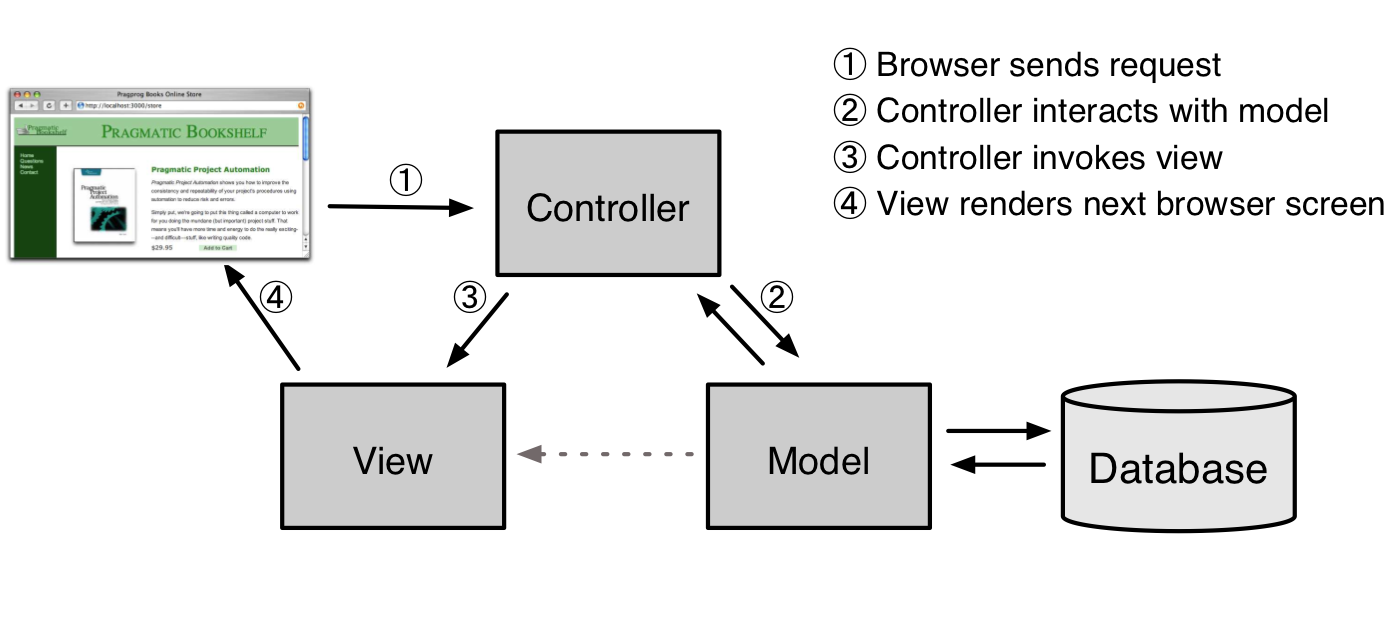
\includegraphics[scale=0.25]{mvc.PNG}
		\caption{Modelo Vista Controlador}
	\label{fig:mvc}
\end{figure}

Los programadores profesionales, suelen escribir tests para simular el comportamiento de la aplicación que se esta desarrollando, para el presente proyecto, se buscaba que el framework tuvieran un soporte para hacer tests, una vez más Rails se ajusta a esas necesidades, pues cuenta con soporte para algunos frameworks para realizar tests, se encuentran; RSpec (utilizada en este proyecto, bajo la filosofía de TDD \footnote{Léase \textbf{TDD} en el glosario}) en donde se escriben los tests, antes de la implementación, Test Unit, Shoulda y Cucumber (BDD\footnote{Léase \textbf{BDD} en el glosario})\\

Se buscaba que la herramienta fuera escrita en un lenguaje de programación orientado a objetos e interpretado, por la necesidad de crear \emph{scripts} que corrieran independiente de la aplicación, como tareas programadas para correr cada cierto tiempo. Las aplicaciones en \emph{Rails} son escritas en el lenguaje de programación \emph{Ruby}, que cumple con lo que se buscaba, y aparte introduce características favorables como metaprogramación, haciendo que el código sea más fácil de entender, leer y/o escribir, programas más cortos en términos de \textbf{LOC}\footnote{Líneas de código, en inglés \emph{Lines of Code}}, para evidenciar esto, a continuación se muestra una porción de código de la aplicación, en la que se define una clase de un Modelo que expresa mucha información en pocas líneas de código y es fácil de entender. \newpage

\begin{verbatim}
class Record < ActiveRecord::Base  

  belongs_to :stock_action

  validates_presence_of :amount
  validates_presence_of :price
  validates_presence_of :variation

  validates_numericality_of :price, :amount, :greater_than => 0
  validates_numericality_of :variation

end
\end{verbatim}

Finalmente, no se pretendía manipular la base de datos directamente, es decir, con código nativo del motor de bases de datos, sino sacar provecho de técnicas como ORM \footnote{Léase \textbf{ORM} en el glosario}, en las que las tablas de las bases de datos son mapeadas a clases, los registros de las tablas son mapeados como objetos, y consecuentemente los campos, se mapean como atributos de los objetos, mientras que existen metodos de clases que se encargan de realizar operaciones a nivel de tablas, dejando como opcional la utilización de código \textbf{SQL} dentro de la aplicación, una vez más \emph{Rails} suple esta necesidad con \textbf{ActiveRecord} ó \textbf{Datamapper}.

\section{¿Por qué Unity3D?}

Actualmente existen posibilidades para el desarrollo de interfaces gráficas de usuario tridimensionales en los navegadores de internet, \textbf{PaperVision3D}\footnote{\textbf{Papervision} es un motor de gráficos para Flash. Aunque todavía está en versión beta, ya se han lanzado algunas aplicaciones que lo utilizan y los resultados son muy prometedores.} (entre otros) es un motor de renderizado 3D en tiempo real, escrito en \textbf{ActionScript 3}\footnote{\textbf{ActionScript} es un lenguaje de programación orientado a objetos (OOP), utilizado en especial en aplicaciones web animadas realizadas en el entorno \textbf{Adobe Flash}}, de código abierto entre otros, que posee las funcionalidades básicas de la computación gráfica tridimensional, creando una ilusión 3D en el motor de renderizado que posee el \emph{Flash Player}. \\

Desafortunadamente el motor de renderizado para \emph{Flash} esta diseñado específicamente para gráficos en 2D. Este es un punto crítico por el cual \emph{Flash} no es técnicamente la mejor opción. La cantidad de fotogramas de contenido 3D renderizados por segundo (FPS)\footnote{Las imágenes por segundo (en inglés más conocido como \emph{frames per second, fps}) es la medida de la frecuencia a la cual un reproductor de imágenes genera distintos fotogramas (\emph{frames}). En informática estos fotogramas están constituídos por un número determinado de pixeles que se distribuyen a lo largo de una red de texturas para determinar un fotograma por segundo.\\
La frecuencia es proporcional al número de pixeles que se deben generar, incidiendo en el rendimiento de la máquina.} suele ser media o baja, en casos reales. La comunidad de desarrolladores del \emph{Flash Player} está desarrollando varios proyectos para poder renderizar 3D en el mismo, existen proyectos privados y de código abierto, entre los que se encuentran: \\
\begin{itemize}
\item[$\bullet$] \emph{Alternativa3D} 
\item[$\bullet$] \emph{Away 3D} 
\item[$\bullet$] \emph{Five3D} 
\item[$\bullet$] \emph{ND3D} 
\item[$\bullet$] \emph{Papervision3D} 
\item[$\bullet$] \emph{Sandy3D} 
\item[$\bullet$] \emph{Wire Engine 3D}
\end{itemize} 
Los cuales usualmente utilizan algoritmos de rasterizado para el proceso de generar una imagen 2D a partir de una escena 3D, consumiendo así en dicho proceso, mucha capacidad computacional.\\

La técnica más utilizada hoy en día para la producción de gráficos 3D en tiempo real es la rasterización. La rasterización es básicamente un proceso de transformación de datos de vectores que se convierten en un conjunto de pixeles (imágenes).\\

En pocas palabras, muchos de los motores de renderizado 3D escritos para trabajar con el \emph{plugin} de \emph{Flash}  utilizan bastante lógica para producir una ilusión 3D sobre 2D debido a que es una de las técnicas mas rápidas, pero, como se mencionó anteriormente, estos motores por mas optimizados que estén, siempre van a depender del renderizado 2D para el cual fue diseñado \emph{Flash} en un principio.\\

\textbf{Unity3D} por su parte también es un \emph{plugin} para navegadores, especializado en la creación de contenido 3D en tiempo real. Técnicamente es la mejor opción para desarrollo 3D, pues dicho \emph{plugin} aprovecha las capacidades de procesamiento de hardware de la tarjeta de video para desplegar contenidos en 3D, permitiendo así optimizar ciclos de procesamiento en el mejoramiento de los FPS de la escena en vez de ejecutar cálculos de conversión de imágenes 3D a 2D, repercutiendo enormemente en la experiencia del usuario.\\

\emph{Unity3D} por su parte es un motor escrito en C/C++ que trabaja con \emph{Mono}\footnote{\textbf{Mono} es el nombre de un proyecto de código abierto iniciado por Ximian y actualmente impulsado por Novell (tras la adquisición de Ximian) para crear un grupo de herramientas libres, basadas en GNU/Linux y compatibles con .NET según lo especificado por el ECMA.} y \emph{PhysX}\footnote{\textbf{PhysX} es un chip y un kit de desarrollo diseñados para llevar a cabo cálculos físicos muy complejos. Conocido anteriormente como la SDK de NovodeX, fue originalmente diseñada por AGEIA y tras la adquisición de AGEIA, es actualmente desarrollado por Nvidia e integrado en sus chip gráficos más recientes.} para crear código multiplataforma, haciendo así practicamente transparente generar ejecutables tanto para MacOSX, Windows, widgets y exportar para Web.\\

Gracias a Mono, es fácil generar ejecutables multiplataforma debido a la arquitectura con la que dicho \emph{framework} trabaja. Figura\ref{fig:mono}\\

\begin{figure}[h]
	\centering
		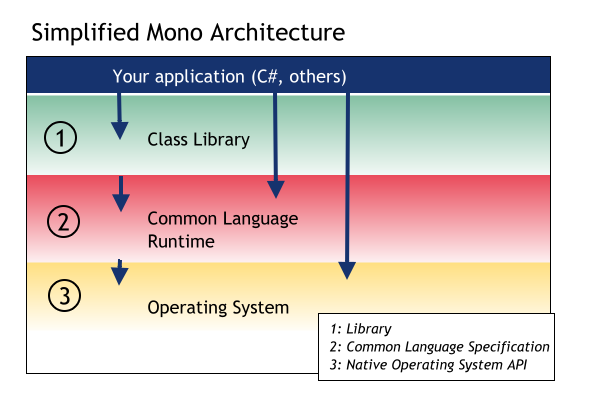
\includegraphics[scale=0.6]{Mono.PNG}
		\caption{Arquitectura general del \emph{framework} Mono}
	\label{fig:mono}
\end{figure}


Por otro lado, \emph{Unity3D} también se aprovecha de la capacidad del motor de física \emph{PhysX} para llevar a cabo cálculos complejos para así alivianar la carga de procesamiento que conlleva un juego/aplicación 3D.\\

Cuando el Motor exporta contenido a Web, dicho contenido se puede comunicar facilmente con \emph{Javascript}, permitiendo así entablar un puente de comunicaciones con \emph{Rails} a través de \emph{Javascript}, factor clave para la visualización de los datos que tiene la aplicación.\\

\section{¿Cómo se complementan estas dos tecnologías?}

Como se justificó en las secciones anteriores, tanto \emph{Rails} como \emph{Unity3D} son herramientas sobre las que se puede desarrollar efectivamente tanto aplicaciones Web convencionales, así como aplicaciones 3D, pero era necesario que ambas tuvieran la forma de recibir y enviar mensajes a través de un protocolo de comunicación, de tal manera que fuera transparente una llamada de una aplicación a la otra como si se tratase de una llamada local.\\

Dicho protocolo de comunicación, fue soportado por \textbf{Javascript} puesto que \emph{Rails} cuenta con una librería bien soportada para convertir datos nativos de \emph{Ruby} a \emph{Javascript} y ya que el contenido generado por \emph{Unity3D} tiene una API accequible escrita en \emph{Javascript} para controlar el estado del contenido dentro del browser, haciendo entonces a \emph{Javascript} la herramienta óptima para comunicar ambas tecnologias.\\



\backmatter

%\scriptsize{



%% \bibitem{Ba97} Barendregt Henk.
%% {\it The Impact of the Lambda Calculus in Logic and Computer Science},
%% The Bulletin of Symbolic Logic. {\bf vol 3}, Number 2, 181-215
%% June 1997.


%% \bibitem{TD} Troelstra A.S y Van Dalen  D. ,
%% {\it Constructivism in mathematics: An introduction},
%% Studies in logic and the foundations of Mathematics. {\bf vol 121,123}
%% 1988.



%% \bibitem{Sth}  Thompson Simon, 
%% Type Theory \& Functional Programming. Addison Wesley, 1991.


%% \bibitem{tcfp} Thompson Simon,
%%  Haskell The Craft of Fucntional Programming, Addison Wesley,
%% Second Edition, 1999.


%% \bibitem{Var82} Vardi M.Y. ,
%% {\it The complexity of relational query languages}. In Proc. 14 th ACM Symp. on Theory
%% of Computing,  1982.


%% \bibitem{Wig60}Wigner  Eugene P., 
%%   {\it The unreasonable effectiveness of mathematics in the natural sciences},
%% Communications in Pure and Applied Mathematics, {\bf vol 13}, No 1, 
%% 1960.


%% \bibitem{Wa00} Wadler Philip,
%% {\it Proofs are Programs:19th Century Logic and 21st Century Computing}. 
%% June 2000, updated November 2000.


%% \bibitem{web2}Isabelle a generic proof assistant,
%% \url{www.cl.cam.ac.uk/research/hvg/Isabelle/}.
%% \bibitem{web1}The coq proof assistant,
%% \url{www.coq.inria.fr}.

%% \end{thebibliography}
\bibliography{tesis}
\bibliographystyle{plain}

\end{document}



